\documentclass[10pt]{beamer}

% preâmbulo
\usepackage[utf8]{inputenc} % ou latin1
\usepackage[T1]{fontenc}
\usepackage[portuges]{babel}
\usepackage{graphicx}
\usepackage{booktabs}
\usepackage{enumerate}
\usepackage{multicol}

\usetheme{Antibes}

\title{Stone Pagamentos\\ Desafio Operações\\ Parte 1}
\author{Marcelo Lima de Moraes}
\date{13 de Junho de 2019}
\begin{document}

\frame{\titlepage}

\begin{frame} 
\frametitle{Sistema de Pagamentos Brasileiro (SPB)}

O SPB compreende as \underline{entidades}, \underline{sistemas} e \underline{procedimentos} relacionados ao \textbf{processamento} e a \textbf{liquidação} de \textbf{operações de transferências de fundos}, \textbf{operações com moeda estrangeira} ou com \textbf{ativos financeiros e valores mobiliários}. Coletivamente, as entidades são chamadas de operadoras de \textbf{Infraestrutura do Mercado Financeiro (IMF)}. Além das IMF, os \textbf{Arranjos} e \textbf{Instituições de Pagamento} também integram o SPB.
\\~\\

O \textbf{Banco Central do Brasil (BACEN)} regula e supervisiona os sistemas de compensação e liquidação, arranjos e instituições de pagamento. Além disso, ele também atua como \textbf{provedor de serviços de liquidação}, operando o \textbf{Sistema de Transferência de Reservas (STR)} e o \textbf{Sistema Especial de Liquidação e Custódia (SELIC)}.
\end{frame}

\begin{frame} 
\frametitle{Infraestruturas do Mercado Financeiro (IMF)}

São integrantes do SPB e estão sujeitas à regulação do \textbf{BACEN}, do Conselho Monetário Nacionao (\textbf{CMN}) e da Comissão de Valores Mobiliários (\textbf{CVM}). São elas os serviços de
\begin{itemize}
	\item Compensação de cheques
	\item Compensação e liquidação de ordens eletrônicas de débito e crédito
	\item Transferências de fundos e de outros ativos financeiros
	\item Compensação e de liquidação de operações com títulos e valores mobiliários
	\item Compensação e de liquidação realizas em bolsas de mercadorias
	\item Futuros
	\item Depósito centralizado
	\item Registro de ativos financeiros e de valores mobiliários
\end{itemize}
\end{frame}

\begin{frame} 
\frametitle{Rede do Sistema Financeiro Nacional (RSFN)}

\begin{figure}[hbtp] % !htb
	\centering
	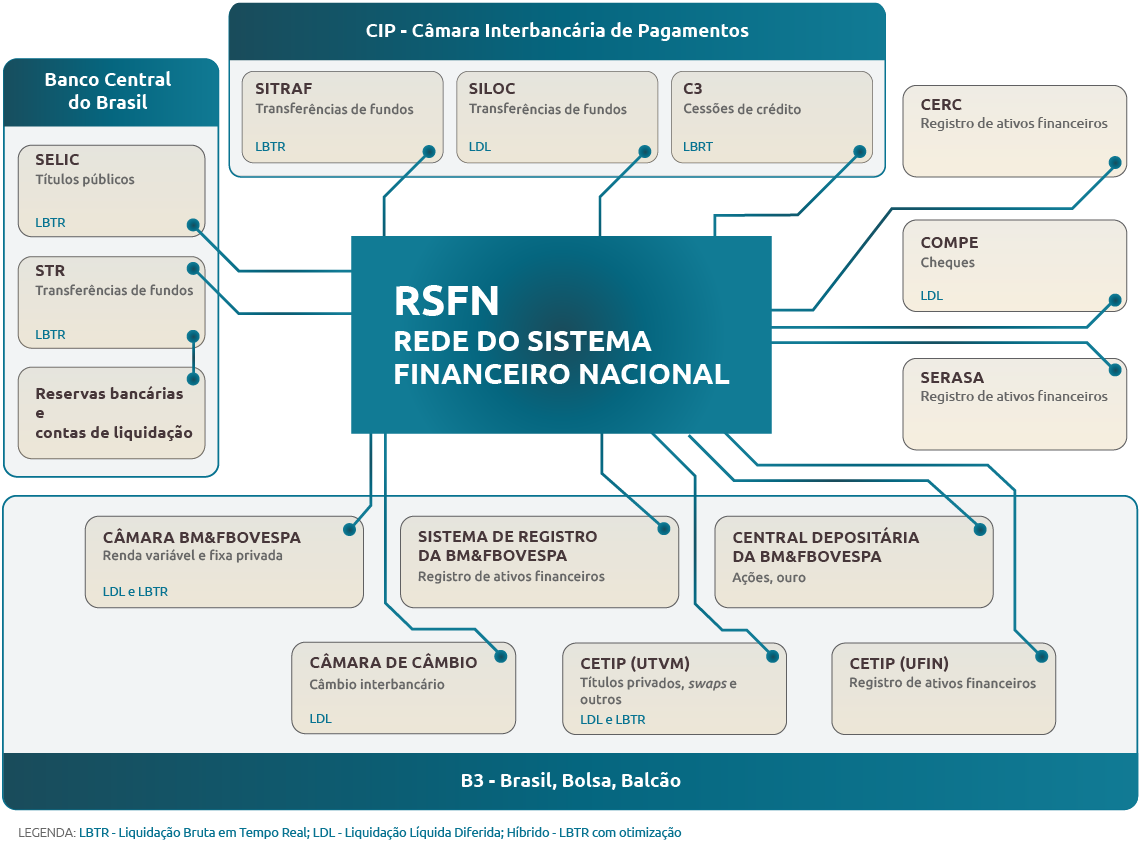
\includegraphics[width=9.75cm]{RSFN.png}
\end{figure}

\end{frame}


\begin{frame} 
\frametitle{Sistema de Transferência de Reservas (STR)}

É o coração do SPB e onde ocorre a \textbf{liquidação final de todas as obrigações} financeiras do país, sendo a \textbf{transferência de fundos via STR irrevogável} e \textbf{lançamento a descoberto (saldo negativo) não permitido}.
\\~\\

Foi instituído pela Circulas nº3100/2002 e opera em \textbf{Liquidação Bruta em Tempo Real (LBTR)}.
\end{frame}

\begin{frame} 
\frametitle{Estrutura do STR}

\begin{figure}[hbtp] % !htb
	\centering
	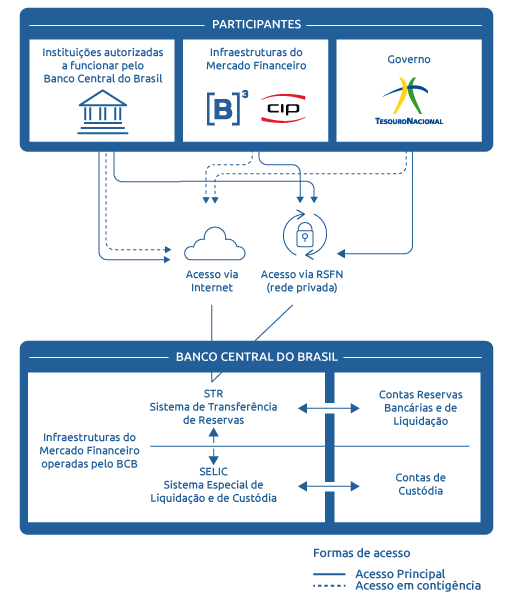
\includegraphics[width=7cm]{estruturaSTR.png}
\end{figure}

\end{frame}

\begin{frame} 
\frametitle{Legislação STR 1}

\begin{itemize}
\item Circular nº3100/2002: Institui o STR e aprova seu regulamento
\item Circular nº3489/2010: Regulamenta aplicativo de acesso ao STR via internet
\item Circular nº3437/2010: Divulga procedimentos para emissão e liquidação de ordem de transferência de fundos agendada no STR
\item Circular nº3525/2011: Esclarece sobre procedimentos para execução da rotina de otimização de liquidação no STR
\item Circular nº3894/2018: Procedimentos a serem observados para a operação de participante em regime de contingência no STR
\item Circular nº3403/2009: Procedimentos para a prestação das informações cadastrais referentes aos responsáveis dos participantes do STR
\item Circular nº3825/2017: Procedimentos atinentes ao monitoramento do STR
\end{itemize}
\end{frame}

\begin{frame} 
\frametitle{Legislação STR 2}

\begin{itemize}
\item Circular nº3217/2005: Procedimentos relativos à cobrança e ao pagamento de tarifas pela utilização do STR
\item Circular nº3514/2011: Procedimentos e horários no âmbito do STR
\item Circular nº3682/2014: Procedimentos operacionais referentes à postergação do horário de fechamento de sessão específica do STR
\item Comunicado nº25268/2014: Divulga alteração de horários para registro e liquidação de ordens de transferência de fundos por clientes
\item Resolução nº2932/2002: Horário de funcionamento e dias
\item Circular nº3930/2019: Divulga as tarifas por utilização do STR de que trata o art. 40 do regulamento do STR anexo à circular nº3100/2002
\end{itemize}
\end{frame}

\begin{frame} 
\frametitle{Legislação, exceto STR}

\begin{enumerate}		
\item Autorização de funcionamento de instituição financeira
\begin{itemize}	
\item Resoluções nº4122/2012, nº4434/2015, e nº4656/2018
\item Circular nº3649/2013.
\end{itemize}
\item Instrumentos de pagamento
\begin{itemize}
\item Circulares nº3115/2002, nº3335/2006, nº3859/2017, nº3532/2011, nº3598/2012, nº3226/2004 e nº3224/2004.
\end{itemize}
\item Arranjos e instituições de pagamento
\begin{itemize}
\item Resolução nº4282/2013
\item Circulares nº3680/2013, nº3681/2013, nº3682/2013 e nº3885/2015.
\end{itemize}
\item Infraestruturas do mercado financeiro
\begin{itemize}
\item Lei nº10214/2001
\item Resolução nº2882/2001
\item Circular nº3057/2001.
\end{itemize}
\item Conta correspondente a moeda eletrônica
\begin{itemize}
\item Circulares nº3704/2014, nº3893/2018 e nº3662/2014.
\end{itemize}
\item Portabilidade de crédito
\begin{itemize}
\item Resoluções nº3401/2006, nº4292/2013, nº3998/2011 e nº3553/2011.
\end{itemize}
\end{enumerate}

\end{frame}

\begin{frame} 
\frametitle{Arranjos de Pagamentos}

São conjuntos de regras e procedimentos que disciplinam a prestação de determinado\textbf{ serviço de pagamento ao público}, conectando os que os aderem.

\begin{figure}[hbtp] % !htb
	\centering
	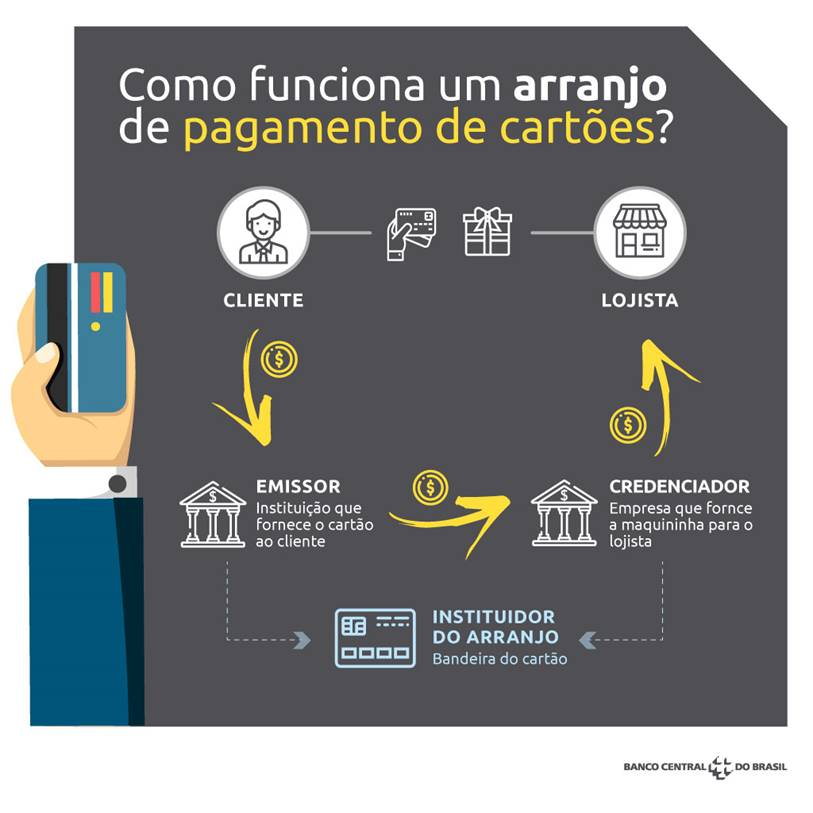
\includegraphics[width=6.4cm]{exemplo_arranjo1.jpg}
\end{figure}

\end{frame}

\begin{frame} 
\frametitle{Arranjos de Pagamentos}

Pessoas Jurídicas (PJs) que executam os serviços de pagamento são chamadas de \textbf{Instituições de Pagamento} e são responsáveis pelo relacionamento com os usuários finais do serviços.
\\~\\

A \textbf{legislação proíbe} que \textbf{instituições de pagamentos} prestem serviços privativos de instituições financeiras, como \textbf{concessão de empréstimos e financiamentos} ou \textbf{disponibilização de conta bancária e de poupança}.

\end{frame}

\begin{frame} 
\frametitle{Contas de Pagamento}

A circular nº3680/2013 dispõe sobre a conta de pagamento utilizada pelas instituições de pagamento. O uso é obrigatório pelas instituições de pagamento emissoras de moeda eletrônica.
\\~\\
\textbf{Titularidade}: usuário final
\\
\textbf{Utilização}: registros de transações de pagamento de usuários finais
\\
\textbf{Uso}: registros de débitos e créditos relativos a transações de pagamento, identificando também o titular
\\~\\
\textbf{Classificação}:
\begin{itemize}
	\item \underline{Pré-Paga}: destinada à execução de transações de pagamento em moeda eletrônica realizadas com base em \textbf{fundos} denominados em reais e \textbf{previamente aportados}
	\item Pós-paga: destinada à execução de transações de pagamento que \textbf{independem do aporte prévio} de recursos
\end{itemize}

\end{frame}

\begin{frame} 
\frametitle{Contas de Pagamento: Resgate e Responsável}

As instituições de pagamento emissoras de moeda eletrônica devem assegurar ao usuário final a \textbf{possibilidade do resgate total}, a \textbf{qualquer tempo}, dos saldos existentes em contas de pagamento pré-pagas.
\\~\\
As instituições de pagamento devem designar, expressamente, um \textbf{Diretor responsável} pelo cumprimento das normas relativas à conta de pagamento

\end{frame}

\begin{frame} 
\frametitle{Contas de Pagamento: Identificação de Informações}

Em contas de pagamento pré-pagas com saldo superior a R\$5000, devem ser realizada a identificação, inclusive com a manutenção, no mínimo, das seguintes informações a serem remetidas ao BACEN:
\\
\begin{itemize}
	\item Pessoa Natural 
	\begin{multicols}{2}
	\begin{itemize}
		\item Nome completo 
		\item Nome completo da mãe
		\item Data de nascimento
		\item CPF 
		\item Endereço residencial
		\item Número de telefone com DDD
	\end{itemize}
 	\end{multicols}
	\item Pessoa Jurídica 
	\begin{multicols}{2}
	\begin{itemize}
		\item Firma ou denominação social e CNPJ
		\item Atividade principal
		\item Forma e data de constituição
		\item CPF e nome completo dos representantes, mandatários ou prepostos autorizados 
	\end{itemize}
	\end{multicols}
\end{itemize}
\\
As informações devem ser atualizadas e deve haver \textbf{testes de verificação} com \textbf{periodicidade máxima de um ano}.

\end{frame}

\begin{frame} 
\frametitle{Contas de Pagamento: Prevenção de Crimes\\Circular nº3461/2009}

Para fins de prevenção e combate às atividades relacionadas com \textbf{crimes de “lavagem” ou ocultação de bens, direito e valores e financiamento do terrorismo}, as instituições devem: 
\begin{itemize}
\item Implementar \textbf{sistemas de gerenciamento de risco} para identificação e avaliação de risco
\item Promover \textbf{medidas de mitigação} proporcionais dos riscos identificados
\end{itemize}

\end{frame}

\begin{frame} 
\frametitle{Cadastro de Clientes do Sistema Financeiro Nacional (CCS)\\Circular nº3347/2007}
\\
O CCS é destinado ao \textbf{registro de informações relativas a correntistas e clientes de instituições financeiras}, das demais \textbf{instituições} por ele autorizadas a funcionar e das \textbf{administradoras de consórcios}, bem como a seus \textbf{representantes legais} ou convencionais.
\\~\\
Quem são os clientes e correntistas?
\\
Quem \textbf{detém a titularidade de contas de depósito ou ativos financeiros sob a forma de bens, direitos e valores}.
\\~\\
\textbf{Atualização}: Diária
\\
\textbf{Base de Dados}: até 10 anos após término de relacionamento
\\
\textbf{Envio de informações}: informações relativas a uma determinada data-base até as 8 horas da correspondente data-movimento.
\end{frame}

\begin{frame} 
\frametitle{Cadastro de Clientes do Sistema Financeiro Nacional (CCS)\\Circular nº3347/2007}

\begin{block}{Definições}
\textbf{Data-base} é a data em que ocorrer o evento objeto da informação a ser prestada, correspondendo às datas do seu início e término (informações sobre relacionamentos), ou à data da sua efetivação (solicitações de detalhamento de informações).
\\
\textbf{Data-movimento} é a data-limite para a remessa de informações ao BACEN, correspondente ao segundo dia útil posterior à data-base (informações sobre o relacionamento) ou ao dia útil subseqüente ao pedido (solicitações de detalhamento de informações).
\end{block}
\\
As informações devem ser remetidas utilizando os documentos 5200, 5201 e 5202 do \textbf{Catálogo de Documentos (Cadoc)} e as instituições devem designar \textbf{diretor responsável} que também pode acumular a atribuição de administração de recursos de terceiros.
\end{frame}

\begin{frame} 
\frametitle{Procedimentos de Manutenção de Recursos em Espécie\\Circular nº3893/2018}

Aplica-se às \textbf{instituições emissoras de moeda eletrônica} e aos titulares de Reservas Bancárias e de Conta de Liquidação, exceto câmaras e prestadores de serviços de compensação e liquidação. Os recursos mantidos no BACEN \textbf{correspondem ao valor do saldo das moedas eletrônicas mantidas em conta de pagamento}.

\end{frame}

\begin{frame} 
\frametitle{Procedimentos de Manutenção de Recursos em Espécie\\Circular nº3893/2018}

\begin{block}{Definições}
	\textbf{Instituição e Emissora de Moeda Eletrônica (IEME)}: gerencia conta de pagamento de usuário final, do tipo pré-paga, e disponibiliza transação de pagamento com base em moeda eletrônica aportada nesta conta.
	\\~\\
	\textbf{Conta Correspondente a Moeda Eletrônica (CCME)}: conta específica mantida no BACEN, de titularidade das instituições de pagamento, das instituições financeiras e das demais instituições autorizadas a funcionar pelo BACEN, quando emissoras de moeda eletrônica, destinada exclusivamente à manutenção dos recursos em espécie correspondentes ao valor do saldo das moedas eletrônicas mantidas em conta de pagamento pré-paga por elas gerenciadas, acrescido dos saldos de moedas eletrônicas em trânsito entre contas de pagamento na mesma instituição de pagamento.
\end{block}

\end{frame}


\begin{frame} 
\frametitle{Procedimentos de Manutenção de Recursos em Espécie\\Circular nº3893/2018}
As \textbf{movimentações de recursos na CCME} são realizadas por meio de mensagens do Grupo de Serviços SME, do Catálogo de Serviços do SFN. O envio das mensagens é feito por meio da \textbf{RSFN} ou pela internet, utilizando o \textbf{STR-Web}. 

\begin{itemize}
\item Alocação dos Recursos: transferência a crédito da CCME 
\begin{itemize}
\item Mensagem “SME0001- IF requisita transferência para depósito em conta específica” 
\item As instituições titulares de Conta de Liquidação podem comandar transferências exclusivamente para a CCME de sua titularidade
\end{itemize}
\item Saque dos Recursos: transferência a débito da CCME
\begin{itemize}
\item Comandada exclusivamente pelo titular da referida conta 
\item Mensagem “SME0002- IEME requisita transferência para saque em conta específica”
\item Caso o titular seja participante do STR os recursos são creditados na conta Reservas Bancárias ou Conta de Liquidação de sua titularidade
\end{itemize}
\end{itemize}

\end{frame}

\begin{frame} 
\frametitle{TED via STR (Recebimento e Envio)\\Circular nº3115/2002}

A TED é uma \textbf{ordem de transferência de fundos interbancária}, inclusive envolvendo transferência por conta de terceiros ou a favor de cliente, \textbf{liquidada por intermédio de um sistema de liquidação de transferência de fundos}, sendo os correspondentes recursos disponíveis para o favorecido.
\\~\\
\textbf{Instituição titular de conta de liquidação escolhe o tipo de liquidação} e pode oferecer a TED como \textbf{remetente dos fundos}.
\\~\\
Apenas bancos comerciais, os bancos múltiplos com carteira comercial, a CEF e as cooperativas de crédito podem executar TED emitida por cliente envolvendo diferentes titulares e receber TED, remetida por conta de instituição, para crédito em conta de cliente.

\end{frame}

\begin{frame} 
\frametitle{TED via STR (Recebimento e Envio): Informações\\Circular nº3115/2002}

Para \textbf{emissão de uma TED} devem ser informados, obrigatoriamente: 
\begin{itemize}
	\item Identificação do emitente no sistema de liquidação de transferência de fundos
	\item Número de inscrição no CNPJ do emitente
	\item Identificação do recebedor no sistema de liquidação de transferência de fundos
	\item Número de inscrição do recebedor no CNPJ
	\item Valor da transferência, em moeda nacional
	\item Data da emissão
\end{itemize}

Para emissão de uma TED por conta de terceiros ou a favor de cliente, devem ser informados, adicionalmente, outros dados. 

\end{frame}

\begin{frame} 
\frametitle{Serviços de Liquidação\\Circular nº3057/2001}

Disciplina o funcionamento dos sistemas operados pelas câmaras e pelos prestadores de serviços de compensação e de liquidação.

Podem ser objetos de liquidação as obrigações oriundas de:
\begin{itemize}
	\item Cheques e outros documentos
	\item Ordens eletrônicas de débito e de crédito
	\item Transferências de fundos e outros ativos financeiros
	\item Operações com títulos e valores mobiliários
	\item Operações realizadas em bolsas de mercadorias e de futuros
	\item Outras operações, inclusive envolvendo derivativos financeiros
\end{itemize}

\end{frame}

\begin{frame} 
\frametitle{Serviços de Liquidação\\Circular nº3057/2001}

\begin{block}{Definições}
	\textbf{Compensação}: processo que envolve a apuração da posição líquida (créditos menos débitos) de cada participante;
	\\~\\
	\textbf{Liquidação}: processo de extinção de obrigações
	\\~\\
	\textbf{Liquidação bruta em tempo real (LBTR)}: liquidação de obrigações, uma a uma, em tempo real
	\\~\\
	\textbf{Liquidação Diferida}: liquidação realizada em momento posterior ao de aceitação das operações que dão origem às correspondentes obrigações
\end{block}

\end{frame}

\begin{frame} 
\frametitle{Serviços de Liquidação\\Circular nº3057/2001}

Sistema de \textbf{Liquidação Diferida}: liquidação precedida de compensação e liquidação financeira interbancária é definitiva no momento em que efetuadas as resultante movimentações nas contas Reservas Bancárias mantidas no BACEN.
\\~\\
Sistema de \textbf{Liquidação Bruta em Tempo Real}: liquidação financeira interbancária deve ser feita diretamente em conta Reservas Bancárias e é definitiva no momento em que efetuadas as movimentações nas contas Reservas Bancárias mantidas no BACEN.
\\~\\
Nos sistemas LBTR de transferência de fundos, a informação neles originada atinente à transferência de fundos somente deve ser fornecida ao beneficiário no momento em que a transferência for definitiva. 

\end{frame}

\end{document}